\documentclass[10pt,a4paper]{article}
\usepackage[UTF8,fontset = windows]{ctex}
\setCJKmainfont[BoldFont=黑体,ItalicFont=楷体]{等线}
\usepackage{amssymb,amsmath,amsfonts,amsthm,mathrsfs,dsfont,graphicx}
\usepackage{ifthen,indentfirst,enumerate,color,titletoc}
\usepackage{tikz}
\usepackage{makecell}
\usetikzlibrary{arrows,calc,intersections,patterns}
\usepackage[bf,small,indentafter,pagestyles]{titlesec}
\usepackage[top=1in, bottom=1in,left=0.8in,right=0.8in]{geometry}
\renewcommand{\baselinestretch}{1.65}
\newtheorem{defi}{定义~}
\newtheorem{eg}{例~}
\newtheorem{ex}{~}
\newtheorem{rem}{注~}
\newtheorem{thm}{定理~}
\newtheorem{coro}{推论~}
\newtheorem{axiom}{公理~}
\newtheorem{prop}{性质~}
\newcommand{\blank}[1]{\underline{\hbox to #1pt{}}}
\newcommand{\bracket}[1]{(\hbox to #1pt{})}
\newcommand{\onech}[4]{\par\begin{tabular}{p{.9\textwidth}}
A.~#1\\
B.~#2\\
C.~#3\\
D.~#4
\end{tabular}}
\newcommand{\twoch}[4]{\par\begin{tabular}{p{.46\textwidth}p{.46\textwidth}}
A.~#1& B.~#2\\
C.~#3& D.~#4
\end{tabular}}
\newcommand{\vartwoch}[4]{\par\begin{tabular}{p{.46\textwidth}p{.46\textwidth}}
(1)~#1& (2)~#2\\
(3)~#3& (4)~#4
\end{tabular}}
\newcommand{\fourch}[4]{\par\begin{tabular}{p{.23\textwidth}p{.23\textwidth}p{.23\textwidth}p{.23\textwidth}}
A.~#1 &B.~#2& C.~#3& D.~#4
\end{tabular}}
\newcommand{\varfourch}[4]{\par\begin{tabular}{p{.23\textwidth}p{.23\textwidth}p{.23\textwidth}p{.23\textwidth}}
(1)~#1 &(2)~#2& (3)~#3& (4)~#4
\end{tabular}}
\begin{document}

必修第一章复习题A组
\begin{enumerate}[1.]
\item 用列举法表示下列集合:\\
(1) 十二生肖组成的集合;\\
(2) 中国国旗上所有颜色组成的集合.
\item 用描述法表示下列集合:\\
(1) 平面直角坐标系中第一象限的角平分线上的所有点组成的集合;\\
(2) $3$的所有倍数组成的集合.
\item (1) 若$\alpha$: $x^2-5x+6=0$, $\beta$: $x=2$, 则$\alpha$是$\beta$的\blank{50}条件;
(2) 若$\alpha$: 四边形$ABCD$是正方形, $\beta$: 四边形$ABCD$的两条对角线互相垂直平分, 则$\alpha$是$\beta$的\blank{50}条件.
\item 已知方程$x^2+px+4=0$的所有解组成的集合为$A$, 方程$x^2+x+q=0$的所有解组成的集合为$B$, 且$A\cap B=\{4\}$. 求集合$A\cup B$的所有子集.
\item 已知集合$A=(-2, 1)$, $B=(-\infty, -2)\cup [1, +\infty)$. 求: $A\cup B$, $A\cap B$.
\item 已知全集$U=(-\infty, 1)\cup [2, +\infty)$, 集合$A=(-1, 1)\cup [3, +\infty)$. 求$A$.
\item 已知集合$A=\{x|x^2+px+q=0\}$, $B=\{x|x^2-x+r=0\}$, 且$A\cap B=\{-1\}$, $A\cup B=\{-1, 2\}$. 求实数$p$、$q$、$r$的值.
\item 设$a$是实数. 若$x=1$是$x>a$的一个充分条件, 则$a$的取值范围为\blank{50}.
\item 已知陈述句$\alpha$是$\beta$的充分非必要条件. 若集合$M=\{x|x\text{满足}\alpha\}$, $N=\{x|x\text{满足}\beta\}$, 则$M$与$N$的关系为\bracket{20}.
\fourch{$M\subset N$}{$M\supset N$}{$M=N$}{$M\cap N=\varnothing$}
\item 证明: 若梯形的对角线不相等, 则该梯形不是等腰梯形.
\end{enumerate}

必修第一章复习题B组
\begin{enumerate}[1.]
\item 若集合$M=\{a|a=x+\sqrt2y, x,y\in \mathbf{Q}\}$, 则下列结论正确的是\bracket{20}.
\fourch{$M\subseteq \mathbf{Q}$}{$M=\mathbf{Q}$}{$M\supset \mathbf{Q}$}{$M\subset \mathbf{Q}$}
\item 若$\alpha$是$\beta$的必要非充分条件, $\beta$是$\gamma$的充要条件, $\gamma$是$\delta$的必要非充分条件, 则$\delta$是$\alpha$的\blank{50}条件, $\gamma$是$\alpha$的\blank{50}条件.
\item 已知全集$U=\{x|x\text{为不大于}20\text{的素数}\}$. 若$A\cap \overline{B}=\{3, 5\}$, $\overline{A}\cap B=\{7, 19\}$, $\overline{A\cup B}=\{2, 17\}$, 则A=\blank{50} , B=\blank{50}.
\item 已知集合$P=\{x|-2\le x\le 5\}$, $Q=\{x|x\ge k+1\text{且}x\le 2k-1\}$, 且$Q\subseteq P$. 求实数$k$的取值范围.
\item 已知全集$U=\mathbf{R}$, 集合$A=\{x|x\le a-1\}$, $B=\{x|x>a+2\}$, $C=\{x|x<0\text{或}x\ge 4\}$, 且$\overline{A\cup B}\subseteq C$. 求实数$a$的取值范围.
\item 已知集合$A=\{x|(a-1)x^2+3x-2=0\}$. 是否存在这样的实数$a$, 使得集合$A$有且仅有两个子集? 若存在, 求出实数$a$的值及对应的两个子集; 若不存在, 说明理由.
\item 证明: $\sqrt[3]{2}$是无理数. 
\end{enumerate}

必修第一章复习题B组
\begin{enumerate}[1.]
\item 若集合$M=\{a|a=x+\sqrt2y, x,y\in \mathbf{Q}\}$, 则下列结论正确的是\bracket{20}.
\fourch{$M\subseteq \mathbf{Q}$}{$M=\mathbf{Q}$}{$M\supset \mathbf{Q}$}{$M\subset \mathbf{Q}$}
\item 若$\alpha$是$\beta$的必要非充分条件, $\beta$是$\gamma$的充要条件, $\gamma$是$\delta$的必要非充分条件, 则$\delta$是$\alpha$的\blank{50}条件, $\gamma$是$\alpha$的\blank{50}条件.
\item 已知全集$U=\{x|x\text{为不大于}20\text{的素数}\}$. 若$A\cap \overline{B}=\{3, 5\}$, $\overline{A}\cap B=\{7, 19\}$, $\overline{A\cup B}=\{2, 17\}$, 则A=\blank{50} , B=\blank{50}.
\item 已知集合$P=\{x|-2\le x\le 5\}$, $Q=\{x|x\ge k+1\text{且}x\le 2k-1\}$, 且$Q\subseteq P$. 求实数$k$的取值范围.
\item 已知全集$U=\mathbf{R}$, 集合$A=\{x|x\le a-1\}$, $B=\{x|x>a+2\}$, $C=\{x|x<0\text{或}x\ge 4\}$, 且$\overline{A\cup B}\subseteq C$. 求实数$a$的取值范围.
\item 已知集合$A=\{x|(a-1)x^2+3x-2=0\}$. 是否存在这样的实数$a$, 使得集合$A$有且仅有两个子集? 若存在, 求出实数$a$的值及对应的两个子集; 若不存在, 说明理由.
\item 证明: $\sqrt[3]{2}$是无理数. 
\end{enumerate}

必修第一章拓展与思考
\begin{enumerate}[1.]
\item 设$a,b$是正整数. 求证: 若$ab-1$是$3$的倍数, 则$a$与$b$被$3$除的余数相同.
\item 已知非空数集$S$满足: 对任意给定的$x,y\in S$($x,y$可以相同), 有$x+y\in S$且$x-y\in S$.\\
(1) 哪个数一定是$S$中的元素? 说明理由;\\
(2) 若$S$是有限集, 求$S$;\\
(3) 若$S$中最小的正数为$5$, 求$S$.
\end{enumerate}

必修第二章复习题A组
\begin{enumerate}[1.]
\item 设一元二次方程$2x^2-6x-3=0$的两个实根为$x_1,x_2$, 求下列各式的值:\\
(1) $(x_1+1)(x_2+1)$;\\
(2) $(x_1^2-1)(x_2^2-1)$.
\item 设$a>b>0$, 比较$\dfrac{b+2a}{a+2b}$与$\dfrac ab$的值的大小.
\item 已知$x>y$, 求证: $x^3-y^3>x^2y-xy^2$.
\item 若关于x的不等式$(a+1)x-a<0$的解集为$(2,+\infty)$, 求实数$a$的值, 并求不等式$(a-1)x+3-a>0$的解集.
\item 解下列一元二次不等式:\\
(1) $-x^2+11<-2x-4$;\\
(2) $3x^2<13x+10$;\\
(3) $6x+2\ge 5x^2$;\\
(4) $x^2\le 8(1-x)$;\\
(5) $-x^2\ge 9(9-2x)$;\\
(6) $3(x-3)\le x^2$.
\item 试写出一个二次项系数为$1$的一元二次不等式, 使它的解集分别为:\\
(1) $(-\infty, \sqrt 2)\cup  (\sqrt 2, +\infty)$;\\
(2) $[2-\sqrt 3, 2+\sqrt 3]$.
\item 求不等式$5\le x^2-2x+2<26$的所有正整数解.
\item 解下列分式不等式:\\
(1) $\dfrac{2x+1}{x+7}>-3$;\\
(2) $\dfrac{3x}{x^2+2}\ge 1$.
\item 设关于$x$的不等式$a_1x^2+b_1x+c_1>0$与$a_2x^2+b_2x+c_2>0$的解集分别为$A$、$B$,
试用集合运算表示下列不等式组的解集:\\
(1) $\begin{cases} a_1x^2+b_1x+c_1>0, \\ a_2x^2+b_2x+c_2>0;\end{cases}$;\\
(2) $\begin{cases} a_1x^2+b_1x+c_1\le 0, \\ a_2x^2+b_2x+c_2>0;\end{cases}$;\\
(3) $\begin{cases} a_1x^2+b_1x+c_1\le 0, \\ a_2x^2+b_2x+c_2\le 0;\end{cases}$.
\item 解下列含绝对值的不等式:\\
(1) $|2x-1|\le x$;\\
(2) $|2x+1|+|x-2|<8$.
\item 已知$a$、$b$是正数, 求证: $\sqrt{(1+a)(1+b)}\ge 1+\sqrt{ab}$.
\item 如图, 在直角三角形$ABC$中, $AD$垂直于斜边$BC$, 且垂足为$D$. 设$BD$及$CD$的长度分别为$a$与$b$.\\
(1) 求斜边上的高$AD$与中线$AE$的长;\\
(2) 用不等式表示斜边上的高$AD$与中线$AE$长度的大小关系.
\begin{center}
    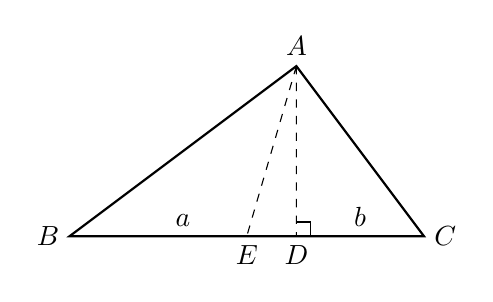
\begin{tikzpicture}[scale = 1.8]
        \draw [thick] (0,0) node [left] {$B$} -- (2.5,0) node [right] {$C$} -- (1.6,1.2) node [above] {$A$} -- cycle;
        \draw [dashed] (1.6,1.2) -- (1.6,0) node [below] {$D$} (1.6,1.2) -- (1.25,0) node [below] {$E$};
        \draw [thin] (1.7,0) -- (1.7,0.1) -- (1.6,0.1);
        \draw (0.8,0) node [above] {$a$} (2.05,0) node [above] {$b$};
    \end{tikzpicture}
\end{center}
\item 如图, 已知直角梯形$ABCD$的顶点$A(a, 0)$、$B(b, 0)$位于$x$轴上, 顶点$C$、$D$落在函数$y=|x|$的图像上, $M$、$N$分别为线段$AB$、$CD$的中点, $O$为坐标原点, $Q$为线段$OC$与线段$MN$的交点.\\
(1) 求中点$M$的坐标, 以及线段$MQ$、$MN$的长度;\\
(2) 用不等式表示$MQ$、$MN$长度的大小关系.
\begin{center}
    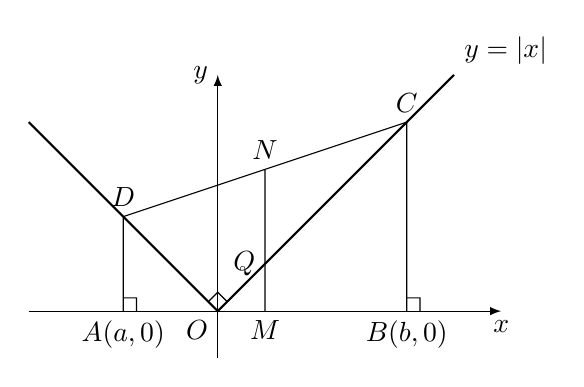
\begin{tikzpicture}[scale = 1.2,>=latex]
        \draw [->] (-2,0) -- (3,0) node [below] {$x$};
        \draw [->] (0,-0.5) -- (0,2.5) node [left] {$y$};
        \draw (0,0) node [below left] {$O$};
        \draw [thick] (-2,2) -- (0,0) -- (2.5,2.5) node [above right] {$y=|x|$};
        \draw [thin] (-0.1,0.1) -- (0,0.2) -- (0.1,0.1) (2.14,0) -- (2.14,0.14) -- (2,0.14) (-0.86,0) -- (-0.86,0.14) -- (-1,0.14);
        \draw (-1,0) node [below] {$A(a,0)$} -- (-1,1) node [above] {$D$} -- (0.5,1.5) node [above] {$N$} -- (2,2) node [above] {$C$} -- (2,0) node [below] {$B(b,0)$} (0.5,1.5) -- (0.5,0.5) node [left] {$Q$} -- (0.5,0) node [below] {$M$}; 
    \end{tikzpicture}
\end{center}
\end{enumerate}

必修第二章复习题B组
\begin{enumerate}[1.]
\item 已知一元二次方程$x^2+px+p=0$的两个实根分别为$\alpha$、$\beta$, 且$\alpha^2$+$\beta^2=3$, 求实数$p$的值.
\item 已知一元二次方程$2x^2-4x+m+3=0$有两个同号实根, 求实数$m$的取值范围.
\item 设$a,b\in \mathbf{R}$, 已知关于$x$的不等式$(a+b)x+(b-2a)<0$的解集为$(1, +\infty)$, 求不等式$(a-b)x+3b-a>0$的解集.
\item 解下列不等式:\\
(1) $-2< \dfrac 1{2x+1}\le 3$;\\
(2) $2<|x+1|\le 3$.
\item 已知集合$A=\{x||x-a|<2\}$, $B=\{x|\dfrac{2x-1}{x+2}<1\}$, 且$A\subseteq B$. 求实数$a$的取值范围.
\item 证明: 若$x>-1$, 则$x+\dfrac 1{x+1}\ge 1$, 并指出等号成立的条件.
\item 设$a$、$b$为正数, 且$a+b=2$. 求$\dfrac 1a+\dfrac 1b$的最小值.
\item 已知$a$、$b$、$c$都是正数, 求证: $\dfrac{b+c}{a}+\dfrac{c+a}{b}+\dfrac{a+b}{c}\ge 6$.
\item 设实数$x$、$y$满足$x+y=1$, 求$xy$的最大值.
\item 已知$a$、$b$为实数, 求证:$|a|+|b| \le |a+b| +|a-b|$, 并指出等号成立的条件.
\item 已知$a$、$b$是实数,\\
(1) 求证: $a^2+ab+b^2\ge 0$, 并指出等号成立的条件;\\
(2) 求证: 如果$a>b$, 那么$a^3>b^3$. 
\end{enumerate}

必修第二章拓展与思考
\begin{enumerate}[1.]
\item 解下列不等式:\\
(1) $\dfrac{3x-11}{x^2-6x+9}\le 1$;\\
(2) $|3-2x| \ge |x+1|$.
\item 已知集合$A=\{x|x^2-2x-3>0\}$, $B=\{x|x^2+px+q\le 0\}$. 若$A\cup B=\mathbf{R}$, 且$A\cap B=[-2,-1)$, 求实数$p$及$q$的值.
\item 已知实数$0<a<b$, 求证: $a<\dfrac{2ab}{a+b}<\sqrt{ab}<\dfrac{a+b}{2}<\sqrt{\dfrac{a^2+b^2}{2}}<b$.
\item 方程$(x-1)(x-2)(x-3)=0$的三个根$1$、$2$、$3$将数轴划分为四个区间, 即$(-\infty, 1)$, $(1, 2)$, $(2, 3)$, $(3, +\infty)$. 试在这四个区间上分别考察$(x-1)(x-2)(x-3)$的
符号, 从而得出不等式$(x-1)(x-2)(x-3)>0$与$(x-1)(x-2)(x-3)<0$的解集.\\
一般地, 对$x_1$、$x_2$、$x_3\in \mathbf{R}$, 且$x_1\le x_2\le x_3$, 试分别求不等式$(x-x_1)(x-x_2)(x-x_3)>0$与$(x-x_1)(x-x_2)(x-x_3)<0$的解集(提示: $x_1$、$x_2$、$x_3$相互之间可能相等, 需要分情况讨论).
\end{enumerate}

必修第三章复习题A组
\begin{enumerate}[1.]
\item 填空题:\\
(1) 若$x^3=5$, 则$x=$\blank{50}; 若$3^x=5$, 则$x=$\blank{50}.\\
(2) 将$\sqrt[4]{a\sqrt[3]{a}} \ (a>0)$化成有理数指数幂的形式为\blank{50}.\\
(3) 若$\log_8x=-\dfrac 23$, 则$x=$\blank{50}.\\
(4) 若$\log_a b\cdot \log_5 a=3$($a>0$且$a\ne 1$), 则$b=$\blank{50}.
\item 选择题:\\
(1) 若$\lg a$与$\lg b$互为相反数, 则有\bracket{20}.
\fourch{$a+b=0$}{$ab=1$}{$\dfrac ab=1$}{以上答案均不对}
(2) 设$a>0$, 下列计算中正确的是\bracket{20}.
\twoch{$a^\frac{2}{3}\cdot a^\frac{3}{2}=a$}{$a^\frac{2}{3}\div a^\frac{3}{2}=a$}{$a^{-4}\cdot a^4=0$}{$(a^\frac{2}{3})^\frac{3}{2}=a$}
\item 已知$10^\alpha=3$, $10^\beta=4$. 求$10^{\alpha+\beta}$及$10^{\alpha-\frac{\beta}2}$的值.
\item 求下列各式的值:\\
(1) $\dfrac{1}{4^x+1}+\dfrac{1}{4^{-x}+1}$;\\
(2) $4^{\sqrt 2+1}\times 2^{3-2\sqrt 2}\times 8^{-\frac 23}$.
\item 已知$\lg a<1$, 化简$\sqrt{(\lg a)2-\lg \dfrac{a^2}{10}}$.
\item 已知$m=\log_2 10$, 求$2^m-m\lg 2-4$的值. 
\end{enumerate}

必修第三章复习题B组
\begin{enumerate}[1.]
\item 填空题:\\
(1) 若$4^x=2^{-12}$, $4^y=\sqrt[3]{32}$, 则$2x-3y=$\blank{50}.\\
(2) 若$\log_3(\log_4 x)=1$, 则$x=$\blank{50}.\\
(3) 若$3^a=7^b=63$, 则$\dfrac 2a+\dfrac 1b$的值为\blank{50}.\\
\item 已知$\log_{18}9=a$, $18^b=5$, 则$\log_{36}45$等于\bracket{20}.
\fourch{$\dfrac{a+b}{2+a}$}{$\dfrac{a+b}{2-a}$}{$\dfrac{a+b}{2a}$}{$\dfrac{a+b}{a^2}$}
\item 设$\log_{0.2}a>0$, $\log_{0.2}b>0$, 且$\log_{0.2}a\cdot \log_{0.2}b=1$, 求$\log_{0.2}(ab)$的最小值.
\item 化简$\dfrac{(1+2^x)(1+2^{2x})(1+2^{4x})(1+2^{8x})(1+2^{16x})}{1-2^{32x}}$(其中$x\ne 0$).
\item 已知$a>1$, $b>0$. 求证: 对任意给定的实数$k$, $a^{2b+k}-a^{b+k}>a^{b+k}-a^k$.
\end{enumerate}

必修第三章拓展与思考
\begin{enumerate}[1.]
\item 甲、乙两人同时解关于$x$的方程: $\log_2x+b+c\log_x2=0$. 甲写错了常数$b$, 得两根
$\dfrac 14$及$\dfrac 18$; 乙写错了常数$c$, 得两根$\dfrac 12$及$64$. 求这个方程的真正根.
\item 已知$a$、$b$及$c$是不为$1$的正数, 且$\lg a+\lg b+\lg c=0$. 求证: $a^{\frac{1}{\lg b}+\frac{1}{\lg c}}\cdot b^{\frac{1}{\lg c}+\frac{1}{\lg a}}\cdot c^{\frac{1}{\lg a}+\frac{1}{\lg b}}=\dfrac{1}{1000}$.
\end{enumerate}

必修第四章复习题A组
\begin{enumerate}[1.]
\item 填空题:\\
(1) 若点$(2, \sqrt 2)$在幂函数$y=x^a$的图像上, 则该幂函数的表达式为\blank{50}; 若点$(2, \sqrt 2)$在指数函数$y=a^x$($a>0$且$a\ne 1$)的图像上, 则该指数函数的表达式为\blank{50}; 若点$(\sqrt 2, 2)$在对数函数$y=\log_a x$($a>0$且$a\ne 1$)的图像上, 则该对数
函数的表达式为\blank{50}.\\
(2) 若幂函数$y=x^k$在区间$(0, +\infty)$上是严格减函数, 则实数$k$的取值范围为\blank{50}.\\
(3) 已知常数$a>0$且$a\ne 1$, 假设无论$a$为何值, 函数$y=a^{x-2}+1$的图像恒经过一
个定点. 则这个点的坐标为\blank{50}.
\item 选择题:\\
(1) 若指数函数$y=a^x$($a>0$且$a\ne 1$)在$\mathbf{R}$上是严格减函数, 则下列不等式中, 一定能成立的是\bracket{20}.
\fourch{$a>1$}{$a<0$}{$a(a-1)<0$}{$a(a-1)>0$}
(2) 在同一平面直角坐标系中, 一次函数$y=x+a$与对数函数$y=\log_ax$($a>0$且$a\ne 1$)的图像关系可能是\bracket{20}.
\fourch{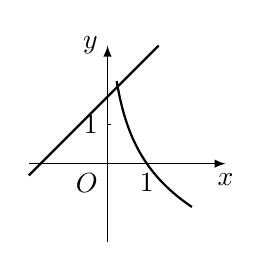
\begin{tikzpicture}[scale = 0.5,>=latex]
    \draw [->] (-2,0) -- (3,0) node [below] {$x$};
    \draw [->] (0,-2) -- (0,3) node [left] {$y$};
    \draw (0,0) node [below left] {$O$};
    \draw (0.1,1) -- (0,1) node [left] {$1$};
    \draw (1,0) node [below] {$1$};
    \draw [thick] (-2,-0.3) -- (1.3,3);
    \draw [thick,domain =-1.1:2.1,samples = 200] plot ({0.5^\x},\x);
\end{tikzpicture}
}{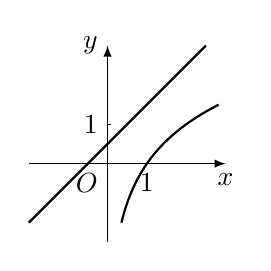
\begin{tikzpicture}[scale = 0.5,>=latex]
    \draw [->] (-2,0) -- (3,0) node [below] {$x$};
    \draw [->] (0,-2) -- (0,3) node [left] {$y$};
    \draw (0,0) node [below left] {$O$};
    \draw (0.1,1) -- (0,1) node [left] {$1$};
    \draw (1,0) node [below] {$1$};
    \draw [thick] (-2,-1.5) -- (2.5,3);
    \draw [thick,domain =1.5:-1.5,samples = 200] plot ({0.5^\x},-\x);
\end{tikzpicture}
}{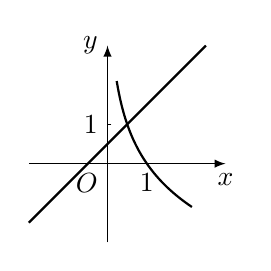
\begin{tikzpicture}[scale = 0.5,>=latex]
    \draw [->] (-2,0) -- (3,0) node [below] {$x$};
    \draw [->] (0,-2) -- (0,3) node [left] {$y$};
    \draw (0,0) node [below left] {$O$};
    \draw (0.1,1) -- (0,1) node [left] {$1$};
    \draw (1,0) node [below] {$1$};
    \draw [thick] (-2,-1.5) -- (2.5,3);
    \draw [thick,domain =-1.1:2.1,samples = 200] plot ({0.5^\x},\x);
\end{tikzpicture}
}{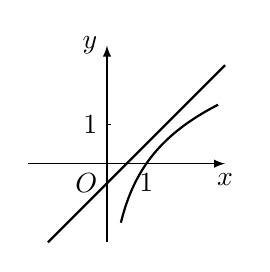
\begin{tikzpicture}[scale = 0.5,>=latex]
    \draw [->] (-2,0) -- (3,0) node [below] {$x$};
    \draw [->] (0,-2) -- (0,3) node [left] {$y$};
    \draw (0,0) node [below left] {$O$};
    \draw (0.1,1) -- (0,1) node [left] {$1$};
    \draw (1,0) node [below] {$1$};
    \draw [thick] (-1.5,-2) -- (3,2.5);
    \draw [thick,domain =1.5:-1.5,samples = 200] plot ({0.5^\x},-\x);
\end{tikzpicture}
}
\item 求下列函数的的定义域:\\
(1) $y=(x-1)^{\frac 52}$;\\
(2) $y=3^{\sqrt{x-1}}$;\\
(3) $y=\lg \dfrac{1+x}{1-x}$.
\item 比较下列各题中两个数的大小:\\
(1) $0.1^{0.7}$与$0.2^{0.7}$;\\
(2) $0.7^{0.1}$与$0.7^{0.2}$;\\
(3) $\log_{0.7}0.1$与$\log_{0.7}0.2$;
\item 设点$(\sqrt 2, 2)$在幂函数$y_1=x^a$的图像上, 点$(-2,\dfrac 14)$在幂函数$y_2=x^b$的图像上. 当$x$取何值时, $y_1=y_2$?
\item 设$a=(\dfrac 23)^x$, $b=x^{\frac 32}$及$c=\log_\frac{2}{3}x$, 当$x>1$时, 试比较$a$、$b$及$c$之间的大小关系.
\item 设常数$a>0$且$a\ne 1$, 若函数$y=\log_a(x+1)$在区间$[0, 1]$上的最大值为$1$, 最小值为$0$, 求实数$a$的值.
\item 如果光线每通过一块玻璃其强度要减少$10\%$, 那么至少需要将多少块这样的玻璃重叠起来, 才能使通过它们的光线强度低于原来的$\dfrac 13$? 
\end{enumerate}

必修第四章复习题B组
\begin{enumerate}[1.]
\item 填空题:\\
(1) 已知$m\in \mathbf{Z}$, 设幂函数$y=x^{m2-4m}$的图像关于原点成中心对称, 且与$x$轴及$y$轴均无交点, 则$m$的值为\blank{50}.\\
(2) 设$a$、$b$为常数, 若$0<a<1$, $b<-1$, 则函数$y=a^x+b$的图像必定不经过第\blank{50}象限.
\item 选择题:\\
(1) 若$m>n>1$, 而$0<x<1$, 则下列不等式正确的是\bracket{20}.
\fourch{$m^x<n^x$}{$x^m<x^n$}{$\log_x m>\log_x n$}{$\log_m x<\log_n x$}
(2) 在同一平面直角坐标系中, 二次函数$y=ax^2+bx$与指数函数$y=(\dfrac ba)^x$的图像关系可能为\bracket{20}.
\fourch{
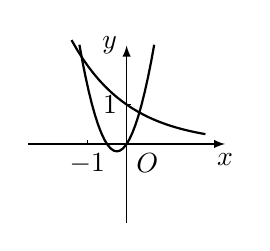
\begin{tikzpicture}[scale = 0.5, >=latex]
    \draw [->] (-2.5,0) -- (2.5,0) node [below] {$x$};
    \draw [->] (0,-2.) -- (0,2.5) node [left] {$y$};
    \draw (0,0) node [below right] {$O$};
    \draw (-1,0.1) -- (-1,0) node [below] {$-1$};
    \draw (0.1,1) -- (0,1) node [left] {$1$};
    \draw [domain = -1.2:0.7,thick] plot (\x,{3*\x * (\x+0.5)});
    \draw [domain = -1.4:2,thick] plot (\x,{(0.5)^\x}); 
\end{tikzpicture}
}{
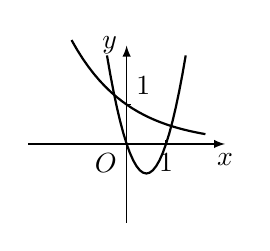
\begin{tikzpicture}[scale = 0.5, >=latex]
    \draw [->] (-2.5,0) -- (2.5,0) node [below] {$x$};
    \draw [->] (0,-2.) -- (0,2.5) node [left] {$y$};
    \draw (0,0) node [below left] {$O$};
    \draw (1,0.1) -- (1,0) node [below] {$1$};
    \draw (0.1,1) -- (0,1) node [above right] {$1$};
    \draw [domain = -0.5:1.5,thick] plot (\x,{3*\x*(\x-1)});
    \draw [domain = -1.4:2,thick] plot (\x,{(0.5)^\x}); 
\end{tikzpicture}
}{
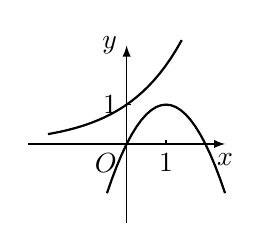
\begin{tikzpicture}[scale = 0.5, >=latex]
    \draw [->] (-2.5,0) -- (2.5,0) node [below] {$x$};
    \draw [->] (0,-2.) -- (0,2.5) node [left] {$y$};
    \draw (0,0) node [below left] {$O$};
    \draw (1,0.1) -- (1,0) node [below] {$1$};
    \draw (0.1,1) -- (0,1) node [left] {$1$};
    \draw [domain = -0.5:2.5,thick] plot ({\x},{-\x*(\x-2)});
    \draw [domain = -1.4:2,thick] plot ({-\x},{(0.5)^\x}); 
\end{tikzpicture}
}{
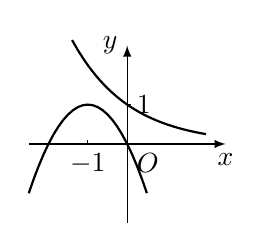
\begin{tikzpicture}[scale = 0.5, >=latex]
    \draw [->] (-2.5,0) -- (2.5,0) node [below] {$x$};
    \draw [->] (0,-2.) -- (0,2.5) node [left] {$y$};
    \draw (0,0) node [below right] {$O$};
    \draw (-1,0.1) -- (-1,0) node [below] {$-1$};
    \draw (0.1,1) -- (0,1) node [right] {$1$};
    \draw [domain = -2.5:0.5,thick] plot ({\x},{-\x*(\x+2)});
    \draw [domain = -1.4:2,thick] plot ({\x},{(0.5)^\x}); 
\end{tikzpicture}   
}
\item 设$a$为常数且$0<a<1$, 若$y=(\log_a \dfrac 35)^x$在$\mathbf{R}$上是严格增函数, 求实数$a$的取值范围.
\item 在同一平面直角坐标系中, 作出函数$y=(\dfrac 12)^x$及$y=x^{\frac 12}$的大致图像, 并求方程$(\dfrac 12)^x=x^{\frac 12}$的解的个数.
\item 已知集合$A=\{y|y=(\dfrac 12)^x,\  x\in [-2, 0)\}$, 用列举法表示集合$B=\{y|y=\log_3x,\  x\in A\text{且}y\in \mathbf{Z}\}$.
\end{enumerate}

必修第四章拓展与思考
\begin{enumerate}[1.]
\item $\log_23$是有理数吗? 请证明你的结论.
\item 仅利用对数函数的单调性和计算器上的乘方功能来确定对数$\log_23$第二位小数的值.
\end{enumerate}

必修第五章复习题A组
\begin{enumerate}[1.]
\item 求函数$y=\dfrac1{2-x}+\sqrt{x^2-1}$的定义域.
\item 判断下列函数$y=f(x)$的奇偶性, 并说明理由:\\
(1) $f(x)=|\dfrac 12 x-3|+|\dfrac 12 x+3|$;\\
(2) $f(x)=x^3+\dfrac 2x$;\\
(3) $f(x)=x^2$, $x\in (k, 2)$(其中常数$k<2$).
\item 已知$m$、$n$是常数, 而函数$y=(m-1)x^2+3x+(2-n)$为奇函数. 求$m$、$n$的值.
\item 求函数$y=x+\dfrac 4x$的单调区间.
\item 分别作出下列函数的大致图像, 并指出它们的单调区间:\\
(1) $y=|x^2-4x|$;\\
(2) $y=2|x|-3$.
\item 已知二次函数$y=f(x)$, 其中$f(x)=ax^2-2ax+3-a \ (a>0)$. 比较$f(-1)$和$f(2)$的大小.
\item 已知$k$是常数, 设$\alpha$、$\beta$是二次方程$x^2-2kx+k+20=0$的两个实根. 问: 当$k$为
何值时, $(\alpha+1)^2+(\beta+1)^2$取到最小值?
\item 邮局规定: 当邮件质量不超过$100$g时, 每$20$g邮费$0.8$元, 且不足$20$g时按$20$g计算; 超过$100$g时, 超过$100$g的部分按每$100$g邮费$2$元计算, 且不足$100$g按$100$g
计算; 同时规定邮件总质量不得超过$2000$g. 请写出邮费关于邮件质量的函数表达式, 并计算$50$g和$500$g的邮件分别收多少邮费.
\item 若函数$y=(a^2+4a-5)x^2-4(a-1)x+3$的图像都在$x$轴上方(不含$x$轴), 求实数$a$的取值范围.
\end{enumerate}

必修第五章复习题B组
\begin{enumerate}[1.]
\item 已知$y=f(x)$是奇函数, 其定义域为$\mathbf{R}$; 而$y=g(x)$是偶函数, 其定义域为$D$. 判断函数$y=f(x)g(x)$的奇偶性, 并说明理由.
\item 设函数$y=x^2+10x-a+3$, 当$x\in [-2, +\infty)$时, 其函数值恒大于等于零. 求实数$a$的取值范围.
\item 已知函数$y=-x^2+2ax+1-a$, $x\in [0, 1]$的最大值为$2$. 求实数$a$的值.
\item 设$f(x)=x^2+ax+1$. 若对任意给定的实数$x$, $f(2+x)=f(2-x)$恒成立, 求实数$a$的值.
\item 已知$y=f(x)$是定义在$(-1, 1)$上的奇函数, 在区间$[0, 1)$上是严格减函数, 且$f(1-a)+f(1-a^2)<0$, 求实数$a$的取值范围.
\item 已知$f(x)=2-x^2$及$g(x)=x$. 定义$h(x)$如下: 当$f(x)\ge g(x)$时, $h(x)=g(x)$; 而当$f(x)<g(x)$时, $h(x)=f(x)$. 求函数$y=h(x)$的最大值.
\end{enumerate}

必修第五章拓展与思考
\begin{enumerate}[1.]
\item 试讨论函数$y=\dfrac{x}{1-x^2}$的单调性.
\item 作出函数$y=(x^2-1)^2-1$的大致图像, 写出它的单调区间, 并证明你的结论.
\item 已知函数$y=f(x)$为偶函数, $y=g(x)$为奇函数, 且$f(x)+g(x)=x^2+2|x-1|+3$. 求$y=f(x)$及$y=g(x)$的表达式.
\item 设函数$y=f(x)$, $x\in \mathbf{R}$的反函数是$y=f^{-1}(x)$.\\
(1) 如果$y=f(x)$是奇函数, 那么$y=f^{-1}(x)$的奇偶性如何?\\
(2) 如果$y=f(x)$在定义域上是严格增函数, 那么$y=f^{-1}(x)$的单调性如何?
\end{enumerate}

必修第六章复习题A组
\begin{enumerate}[1.]
\item 选择题:\\
(1) 与$\sin(\theta -\dfrac\pi 2)$一定相等的是\bracket{20}.
\fourch{$\sin(\dfrac{3\pi}2-\theta)$}{$\cos(\theta -\dfrac{\pi}2)$}{$\cos (2\pi -\theta)$}{$\sin (\theta +\dfrac\pi 2)$}
(2) 当$0<\alpha<\dfrac\pi 4$时, 化简$\sqrt{1-\sin 2\alpha}$的结果是\bracket{20}.
\fourch{$\cos \alpha$}{$\sin \alpha-\cos \alpha$}{$\cos\alpha-\sin\alpha$}{$\sin\alpha+\cos\alpha$}
\item 填空题:\\
(1) 若$\theta$为锐角, 则$\log_{\sin \theta} (1+\cot^2\theta)=$\blank{50};\\
(2) 若$-\dfrac\pi 2<\alpha<0$, 则点$(\cot \alpha, \cos \alpha)$必在第\blank{50}象限;\\
(3) 若$\sin (\pi -\alpha)=\dfrac 23$, $\alpha\in (\dfrac\pi 2, \pi)$, 则$\sin 2\alpha=$\blank{50}.
\item 已知圆$O$上的一段圆弧长等于该圆的内接正方形的边长, 求这段圆弧所对的圆心角的弧度.
\item 已知角$\alpha$的终边经过点$P(3a, 4a)$($a\ne 0$), 求$\sin \alpha$、$\cos \alpha$和$\tan \alpha$.
\item 化简:\\
(1) $\dfrac{\sin (\theta -5\pi )}{\tan (3\pi -\theta )}\cdot \dfrac{\cot (\dfrac\pi 2-\theta )}{\tan (\theta -\dfrac{3\pi} 2)}\cdot \dfrac{\cos (8\pi -\theta )}{\sin(-\theta-4\pi)}$;\\
(2) $\sin (\theta -\dfrac\pi 4)+\cos (\theta +\dfrac\pi 4)$.
\item 已知$\tan \alpha=3$, 求$\dfrac 1{\sin^2\alpha+2\sin \alpha\cos \alpha}$的值.
\item 在$\triangle ABC$中, 已知$a=5$, $b=4$, $A=2B$. 求$\cos B$.
\item 已知$\triangle ABC$的面积为$S$, 求证:\\
(1) $S=\dfrac{a^2\sin B\sin C}{2\sin (B+C)}$;\\
(2) $S=\dfrac{a^2}{2(\cot B+\cot C)}$.
\item (1) 已知$\sin \alpha=\dfrac{\sqrt 5}5$, $\sin \beta=\dfrac{\sqrt {10}}{10}$, 且$\alpha$及$\beta$都是锐角. 求$\alpha+\beta$的值;\\
(2) 在$\triangle ABC$中, 已知$\tan A$与$\tan B$是方程$x^2-6x+7=0$的两个根, 求$\tan C$.
\item 证明: $(\sin \alpha+\sin \beta)^2+(\cos \alpha+\cos \beta)^2=4\cos^2\dfrac{\alpha-\beta}{2}$. 
\end{enumerate}

必修第六章复习题B组
\begin{enumerate}[1.]
\item 选择题:\\
(1) 若$0<x<\dfrac\pi 4$, 且$\lg (\sin x+\cos x)=\dfrac12(3\lg 2-\lg 5)$, 则$\cos x-\sin x$的值为\bracket{20}.
\fourch{$\dfrac{\sqrt{6}}3$}{$\dfrac{\sqrt{3}}2$}{$\dfrac{\sqrt{10}}5$}{$\dfrac{\sqrt{5}}4$}
(2) 下列命题中, 真命题为\bracket{20}.
\onech{若点$P(a, 2a)$($a\ne 0$)为角$\alpha$的终边上一点, 则$\sin \alpha=\dfrac{2\sqrt 5}5$}
{同时满足$\sin \alpha=\dfrac 12$, $\cos \alpha=\dfrac{\sqrt3}2$的角$\alpha$有且只有一个}
{如果角$\alpha$满足$-3\pi <\alpha<-\dfrac 52\pi$, 那么角$\alpha$是第二象限的角}
{$\tan x=-\sqrt 3$的解集为$\{x|x=k\pi -\dfrac\pi 3, \  k\in \mathbf{Z}\}$}
\item 填空题:\\
(1) 在$\triangle ABC$中, 若$a^2+b^2+ab=c^2$, 则$C=$\blank{50};\\
(2) 若$\sin \theta =a$, $\cos \theta =-2a$, 且$\theta$为第四象限的角, 则实数$a=$\blank{50}.\\
\item 已知$\sin \alpha=a\sin \beta$, $b\cos \alpha=a\cos \beta$, 且$\alpha$及$\beta$均为锐角, 求证: $\cos \alpha= \sqrt{\dfrac{a^2-1}{b^2-1}}$.
\item 已知$0<\alpha<\dfrac\pi 2<\beta<\pi$, 且$\cos \beta=-\dfrac13$, $\sin (\alpha+\beta)=\dfrac79$, 求$\sin \alpha$的值.
\item 已知$\pi <\alpha<\dfrac{3\pi} 2$, $\pi <\beta<\dfrac{3\pi} 2$, 且$\sin \alpha=-\dfrac{\sqrt 5}5$, $\cos \beta=-\dfrac{\sqrt 10}10$. 求$\alpha-\beta$的值.
\item 已知$(1+\tan \alpha)(1+\tan \beta)=2$, 且$\alpha$及$\beta$都是锐角. 求证: $\alpha+\beta=\dfrac\pi 4$.
\item 已知$\alpha$是第二象限的角, 且$\sin \alpha=\dfrac{\sqrt {15}}4$. 求$\dfrac{\sin (\alpha+\pi 4)}{1+\sin 2\alpha+\cos 2\alpha}$的值.
\item 证明:\\
(1) $\dfrac{2(1+\sin 2\alpha)}{1+\sin 2\alpha+\cos 2\alpha}=1+\tan \alpha$;\\
(2) $2\sin \alpha+\sin 2\alpha=\dfrac{2\sin^3\alpha}{1-\cos \alpha}$.
\item 根据下列条件, 分别判断三角形$ABC$的形状:\\
(1) $\sin C+\sin (B-A)=\sin 2A$;\\
(2) $\dfrac{\tan A}{\tan B}=\dfrac{a^2}{b^2}$.
\item 在$\triangle ABC$中, 求证: $\tan \dfrac A2\tan \dfrac B2+\tan \dfrac B2\tan\dfrac C2+\tan\dfrac C2\tan\dfrac A2=1$.
\end{enumerate}

必修第六章拓展与思考
\begin{enumerate}[1.]
\item (1) 完成下表($\theta$为弧度数):
\begin{center}
\begin{tabular}{|c|p{.15\textwidth}<{\centering}|p{.15\textwidth}<{\centering}|p{.15\textwidth}<{\centering}|p{.15\textwidth}<{\centering}|p{.15\textwidth}<{\centering}|}
    \hline
    $\theta$ & $1$ & $0.5$ & $0.1$ & $0.01$ & $0.001$\\ \hline
    $\sin\theta$ & & & & &\\ \hline
    $\dfrac{\sin\theta}{\theta}$ & & & & &\\ \hline
\end{tabular}
\end{center}
(2) 观察上表中的数据, 你能发现什么规律?\\
(3) 已知$0<\theta <\dfrac \pi 2$, 利用图形面积公式证明$\sin \theta <\theta <\tan \theta$, 并应用该公式说明(2)中猜想的合理性.
\item 在$\triangle ABC$中, 已知$A=30^\circ$, $b=18$. 分别根据下列条件求$B$:\\
(1) \textcircled{1} $a=6$, \textcircled{2} $a=9$, \textcircled{3} $a=13$, \textcircled{4} $a=18$, \textcircled{5} $a=22$;\\
(2) 根据上述计算结果, 讨论使$B$有一解、两解或无解时$a$的取值情况.
\item (1) 根据$\cos 54^\circ=\sin 36^\circ$和三倍角公式, 求$\sin 18^\circ$的值;\\
(2) 你还能使用其他方法求$\sin 18^\circ$的值吗? 若能, 请给出你的求法.
\item 如图, 要在$A$和$D$两地之间修建一条笔直的隧道, 现在从$B$地和$C$地测量得到: $\angle DBC=24.2^\circ$, $\angle DCB=35.4^\circ$, $\angle DBA=31.6^\circ$, $\angle DCA=17.5^\circ$. 试求$\angle DAB$以确定隧道$AD$的方向(结果精确到$0.1^\circ$).
\begin{center}
    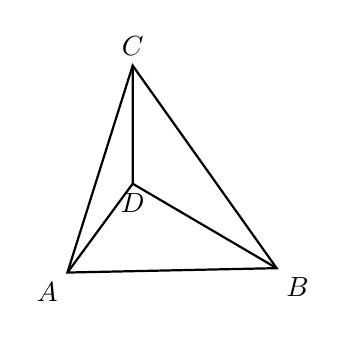
\begin{tikzpicture}
        \draw (0,0) node [below] {$D$} coordinate (D) (0,1.5) node [above] {$C$} coordinate (C) (-0.8287,-1.12831) node [below left] {$A$} coordinate (A) (1.82829,-1.07265) node [below right] {$B$} coordinate (B);
        \draw [thick] (A) -- (B) -- (C) -- cycle;
        \draw [thick] (D) -- (A) (D) -- (B) (D) -- (C);
    \end{tikzpicture}
\end{center}


\begin{center}
    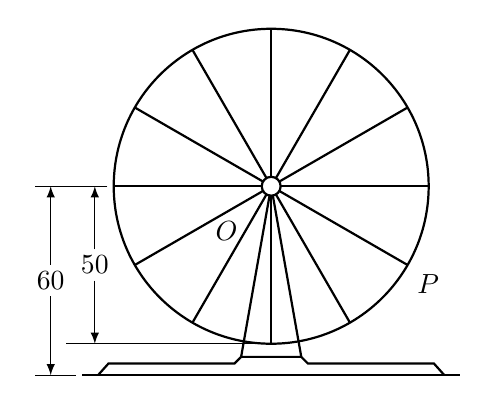
\begin{tikzpicture}[>=latex,scale = 0.4]
        \draw [thick] (0,0) circle (0.3) (0,0) circle (5);
        \foreach \i in {0,30,...,330}{\draw [thick] (\i:0.3) -- (\i:5);};
        \draw [thick] (-80:0.3) -- (-80:5.5) coordinate (R) (-100:0.3) -- (-100:5.5) coordinate (L) (L) -- (R);
        \draw [thick] (L) --++ (-135:0.3) --++ (-4,0) -- (-5.5,-6) (R) --++ (-45:0.3) --++ (4,0) -- (5.5,-6); 
        \draw [thick] (-6,-6) -- (6,-6);
        \draw (-6.2,-6) -- (-7.5,-6) (-5.2,0) -- (-7.5,0) (0,-5) -- (-6.5,-5);
        \draw [->] (-5.6,-2) -- (-5.6,0);
        \draw [->] (-5.6,-3) -- (-5.6,-5);
        \draw (-5.6,-2.5) node {$50$};
        \draw [->] (-7,-2.5) -- (-7,0);
        \draw [->] (-7,-3.5) -- (-7,-6);
        \draw (-7,-3) node {$60$};
        \draw (225:2) node {$O$};
        \draw (-30:5) node [below right] {$P$};
    \end{tikzpicture}
\end{center}

\begin{center}
    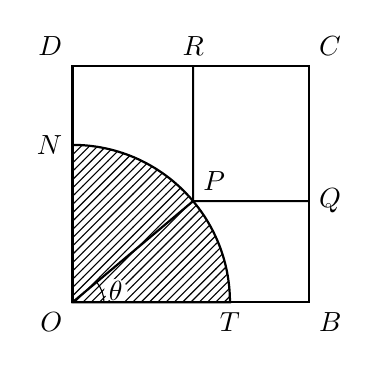
\begin{tikzpicture}
        \begin{scope}[even odd rule]
            \clip (0,0) rectangle (3,3) (0.55,0.15) circle (0.15);
            \fill [pattern = {north east lines}] (0,0) -- (2,0) arc (0:90:2) -- cycle;
        \end{scope}

        \draw [thick] (0,0) node [below left] {$O$} -- (3,0) node [below right] {$B$} -- (3,3) node [above right] {$C$} -- (0,3) node [above left] {$D$} -- cycle;
        \draw [thick] (0,0) -- (40:2) node [above right] {$P$} -- (3,{2*sin(40)}) node [right] {$Q$} (40:2) -- ({2*cos(40)},3) node [above] {$R$};
        \draw [thick] (0,0) -- (2,0) node [below] {$T$} arc (0:90:2) node [left] {$N$} -- cycle;
        \draw (0.4,0) arc (0:40:0.4) (0.55,0.15) node {$\theta$};
    \end{tikzpicture}
\end{center}

\begin{center}
    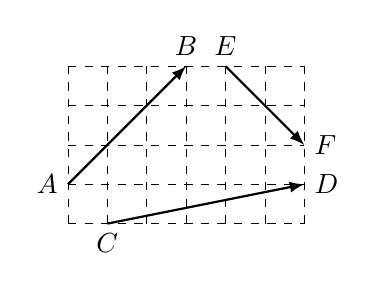
\begin{tikzpicture}[>=latex,scale = 0.5]
        \foreach \i in {0,1,...,4} {\draw [dashed, very thin] (0,\i) -- (6,\i);};
        \foreach \i in {0,1,...,6} {\draw [dashed, very thin] (\i,0) -- (\i,4);};
        \draw [thick,->] (0,1) node [left] {$A$} -- (3,4) node [above] {$B$};
        \draw [thick,->] (1,0) node [below] {$C$} -- (6,1) node [right] {$D$};
        \draw [thick, ->] (4,4) node [above] {$E$} -- (6,2) node [right] {$F$};       
    \end{tikzpicture}
\end{center}

\begin{center}
    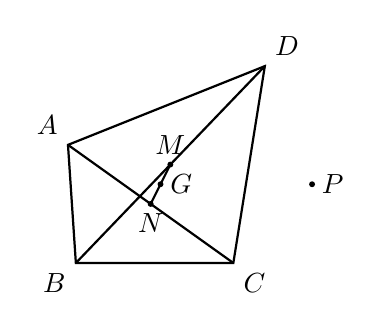
\begin{tikzpicture}
        \draw [thick] (0,0) node [below left] {$B$} coordinate (B) -- (2,0) node [below right] {$C$} coordinate (C) -- (2.4,2.5) node [above right] {$D$} coordinate (D) -- (-0.1,1.5) node [above left] {$A$} coordinate (A) -- cycle;
        \draw [thick] (A) -- (C) (B) -- (D);
        \filldraw ($(B)!0.5!(D)$) circle (0.03) node [above] {$M$} coordinate (M);
        \filldraw ($(A)!0.5!(C)$) circle (0.03) node [below] {$N$} coordinate (N);
        \filldraw ($(M)!0.5!(N)$) circle (0.03) node [right] {$G$} coordinate (G);
        \filldraw (3,1) circle (0.03) node [right] {$P$};
        \draw [thick] (M) -- (N);
    \end{tikzpicture}
\end{center}

\begin{center}
    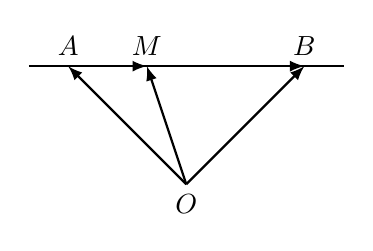
\begin{tikzpicture}[>=latex]
        \draw [thick] (-0.5,0) -- (3.5,0);
        \draw [->,thick] (1.5,-1.5) node [below] {$O$}-- (0,0) node [above] {$A$};
        \draw [->,thick] (1.5,-1.5) -- (3,0);
        \draw [->,thick] (1.5,-1.5) -- (1,0);
        \draw [->,thick] (0,0) -- (1,0) node [above] {$M$};
        \draw [->,thick] (1,0) -- (3,0) node [above] {$B$};
    \end{tikzpicture}
\end{center}

\begin{center}
    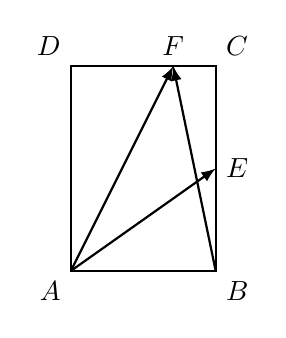
\begin{tikzpicture}[>=latex,thick,scale = 1.3]
        \draw (0,0) node [below left] {$A$} rectangle ({sqrt(2)},2) node [above right] {$C$};
        \draw [->,thick] (0,0) -- ({sqrt(2)},1) node [right] {$E$};
        \draw [->] (0,0) -- (1,2) node [above] {$F$};
        \draw [->] ({sqrt(2)},0) node [below right] {$B$} -- (1,2);
        \draw (0,2) node [above left] {$D$};
    \end{tikzpicture}
\end{center}

\begin{center}
    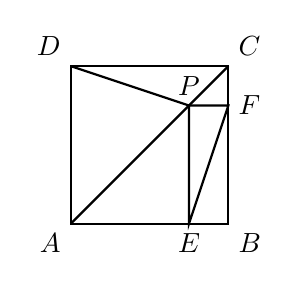
\begin{tikzpicture}[thick]
        \draw (0,0) node [below left] {$A$} rectangle (2,2) node [above right] {$C$};
        \draw (0,2) node [above left] {$D$} -- (1.5,1.5) node [above] {$P$};
        \draw (1.5,1.5) -- (1.5,0) node [below] {$E$} -- (2,1.5) node [right] {$F$} -- cycle;
        \draw (2,0) node [below right] {$B$};
        \draw (0,0) -- (2,2);
    \end{tikzpicture}
\end{center}

\begin{center}
    \begin{tikzpicture}[thick,>=latex,scale = 1.5]
        \fill [fill = gray!20] (0,0.3) -- (0,1.4) -- (3,1.7) -- (3,0.6) -- cycle;
        \draw (0,1.4) -- (3,1.7) (0,0.3) -- (3,0.6);
        \draw [->] (0.6,1) node [below left] {$M$} -- (3,1);
        \draw [dashed,thin] (0,1) -- (0.6,1);
        \draw [->] (0.6,1) --++ (30:1.6) node [above right] {$\overrightarrow{f_1}$};
        \draw [->] (0.6,1) --++ ({2.4-1.6*cos(30)},{-1.6*sin(30)}) node [below right] {$\overrightarrow{f_2}$};
        \draw (2.2,1) node [above] {前进方向};
    \end{tikzpicture}
\end{center}

\begin{center}
    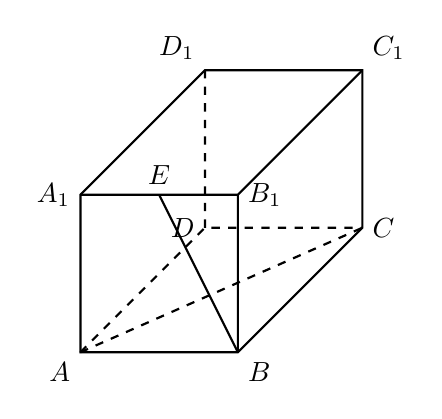
\begin{tikzpicture}[thick]
        \draw (0,0) node [below left] {$A$} coordinate (A) --++ (2,0) node [below right] {$B$} coordinate (B) --++ (45:{2*sqrt(5)/2}) node [right] {$C$} coordinate (C)
        --++ (0,2) node [above right] {$C_1$} coordinate (C1)
        --++ (-2,0) node [above left] {$D_1$} coordinate (D1) --++ (225:{2*sqrt(5)/2}) node [left] {$A_1$} coordinate (A1) -- cycle;
        \draw (A) ++ (2,2) node [right] {$B_1$} coordinate (B1) -- (B) (B1) --++ (45:{2*sqrt(5)/2}) (B1) --++ (-2,0);
        \draw [dashed] (A) --++ (45:{2*sqrt(5)/2}) node [left] {$D$} coordinate (D) --++ (2,0) (D) --++ (0,2);
        \draw ($(A1)!0.5!(B1)$) node [above] {$E$} -- (B);
        \draw [dashed] (A) -- (C);
    \end{tikzpicture}
\end{center}

\begin{center}
    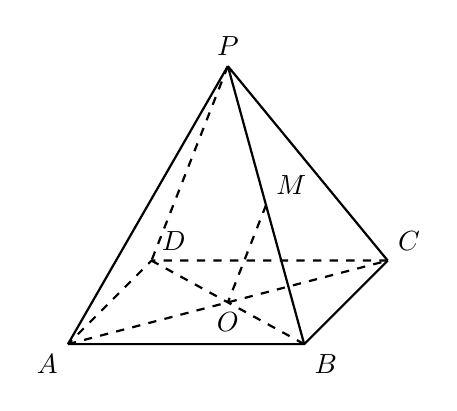
\begin{tikzpicture}[thick]
        \draw (0,0) node [below left] {$A$} coordinate (A) -- (3,0) node [below right] {$B$} coordinate (B)--++ (45:1.5) node [above right] {$C$} coordinate (C);
        \draw [dashed] (C) --++ (-3,0) node [above right] {$D$} coordinate (D) -- (A);
        \draw [dashed] (A) -- (C) (B) -- (D);
        \draw ($(A)!0.5!(C)$) node [below] {$O$} coordinate (O) ++ (0,3) node [above] {$P$} coordinate (P);
        \draw (P) -- (A) (P) -- (B) (P) -- (C);
        \draw ($(P)!0.5!(B)$) node [above right] {$M$} coordinate (M);
        \draw [dashed] (M) -- (O) (P) -- (D);
    \end{tikzpicture}
\end{center}

\begin{center}
    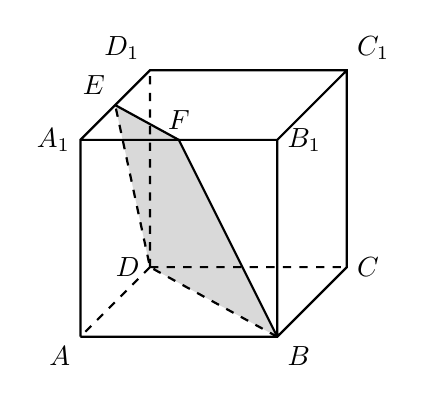
\begin{tikzpicture}[thick]
        \path (0,0) node [below left] {$A$} coordinate (A) --++ (2.5,0) node [below right] {$B$} coordinate (B) --++ (45:{2.5/2}) node [right] {$C$} coordinate (C)
        --++ (0,2.5) node [above right] {$C_1$} coordinate (C1)
        --++ (-2.5,0) node [above left] {$D_1$} coordinate (D1) --++ (225:{2.5/2}) node [left] {$A_1$} coordinate (A1) -- cycle;
        \path (A) ++ (2.5,2.5) node [right] {$B_1$} coordinate (B1) -- (B) (B1) --++ (45:{2.5/2}) (B1) --++ (-2.5,0);
        \path [dashed] (A) --++ (45:{2.5/2}) node [left] {$D$} coordinate (D) --++ (2.5,0) (D) --++ (0,2.5);
        \draw ($(A1)!0.5!(D1)$) node [above left] {$E$} coordinate (E) ($(A1)!0.5!(B1)$) node [above] {$F$} coordinate (F);
        \fill [gray!30] (B) -- (D) -- (E) -- (F);
        \draw (B) -- (F) -- (E);
        \draw [dashed] (B) -- (D) -- (E) (D) -- (C) (D) -- (A) (D) -- (D1);
        \draw (A) -- (B) -- (C) -- (C1) -- (D1) -- (A1) -- (A) (B1) -- (A1) (B1) -- (C1) (B1) -- (B);
    \end{tikzpicture}
\end{center}

\begin{center}
    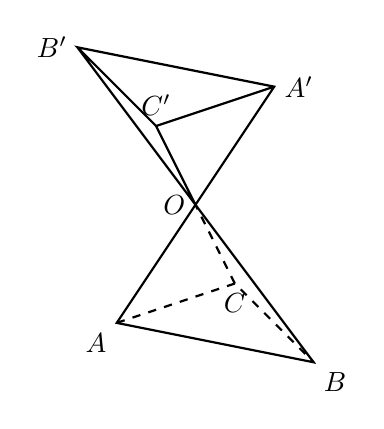
\begin{tikzpicture}[thick]
        \draw (0,0) node [below left] {$A$} coordinate (A);
        \draw (2.5,-0.5) node [below right] {$B$} coordinate (B);
        \draw (1.5,0.5) node [below] {$C$} coordinate (C);
        \draw (1,1.5) node [left] {$O$} coordinate (O);
        \draw (A) -- (B) -- (O) -- cycle;
        \draw [dashed] (A) -- (C) -- (B) (C) -- (O);
        \draw ($(O)!-1!(C)$) node [above] {$C'$} coordinate (C1);
        \draw ($(O)!-1!(A)$) node [right] {$A'$} coordinate (A1);
        \draw ($(O)!-1!(B)$) node [left] {$B'$} coordinate (B1);
        \draw (O) -- (A1) -- (B1) -- (C1) -- (O) (A1) -- (C1) (B1) -- (O);
    \end{tikzpicture}
\end{center}

\begin{center}
    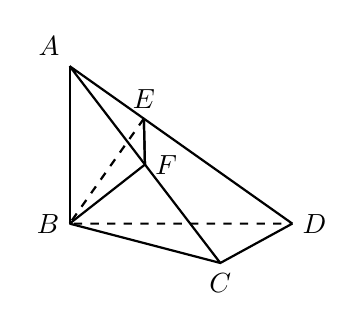
\begin{tikzpicture}[thick,scale = 2]
        \draw (0,0) node [left] {$B$} coordinate (B) -- (0,1) node [above left] {$A$} coordinate (A);
        \draw ({sqrt(2)/2},0) ++ (-45:{sqrt(2)/4}) coordinate (C) node [below] {$C$};
        \draw ({sqrt(2)},0) node [right] {$D$} coordinate (D) -- (C) -- (B) (A) -- (C) (A) -- (D);
        \draw ($(A)!{1/3}!(D)$) node [above] {$E$} coordinate (E) -- ($(A)!0.5!(C)$) node [right] {$F$} coordinate (F);
        \draw (E) -- (F) -- (B);
        \draw [dashed] (E) -- (B) -- (D);
    \end{tikzpicture}
\end{center}

\begin{center}
    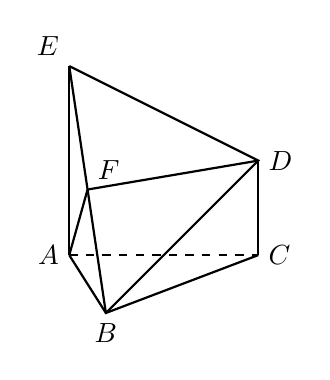
\begin{tikzpicture}[thick,scale = 1.2]
        \draw (0,0) node [left] {$A$} coordinate (A) -- (0,2) node [above left] {$E$} coordinate (E);
        \draw (2,0) node [right] {$C$} coordinate (C) -- (2,1) node [right] {$D$} coordinate (D);
        \draw (1,0) ++ (-135:{sqrt(3)/2}) node [below] {$B$} coordinate (B) -- (E) (B) -- (D) -- (E) ;
        \draw ($(E)!0.5!(B)$) node [above right] {$F$} coordinate (F) -- (A) (F) -- (D);
        \draw [dashed] (A) -- (C);
        \draw (A) -- (B) -- (C);
    \end{tikzpicture}
\end{center}

\begin{center}
    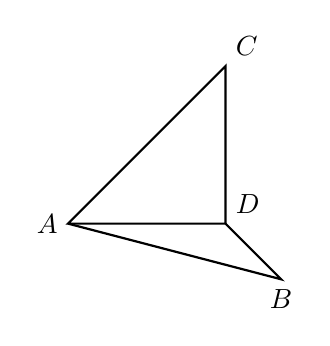
\begin{tikzpicture}[thick]
        \draw (0,0) node [left] {$A$} coordinate (A) -- (2,0) node [above right] {$D$} coordinate (D) -- (2,2) node [above right] {$C$} coordinate (C) -- cycle;
        \draw (2,0) --++ (-45:1) node [below] {$B$} coordinate (B) -- (A);
    \end{tikzpicture}
\end{center}

\begin{center}
    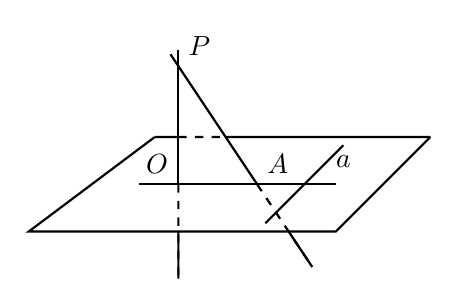
\begin{tikzpicture}[thick]
        \draw (-0.5,0) -- (0,0) node [above left] {$O$} -- (1,0) node [above right] {$A$} coordinate (A) -- (2,0);
        \draw (0,0) coordinate (O) -- (0,1.7) (0,1.5) node [above right] {$P$} coordinate (P);
        \draw ($(P)!{-0.1}!(A)$) -- (A);
        \draw (1.6,0) ++ (45:0.7) node [below] {$a$} --++ (225:1.4);
        \draw (0,-1.2) coordinate (X);
        \draw ($(A)!{-0.7}!(P)$) coordinate (Y);
        \draw (-0.3,0.6) -- (-1.9,-0.6) -- (2,-0.6) -- (3.2,0.6);
        \path [name path=line1] (O) -- (X);
        \path [name path=line2] (A) -- (Y);
        \path [name path=line3] (O) -- (P);
        \path [name path=line4] (A) -- (P);
        \path [name path=under_line] (-1.6,-0.6) -- (2,-0.6);
        \path [name path=above_line] (-0.3,0.6) -- (3.2,0.6);
        \path [name intersections={of = line1 and under_line, by=U}];
        \path [name intersections={of = line2 and under_line, by=V}];
        \path [name intersections={of = line3 and above_line, by=S}];
        \path [name intersections={of = line4 and above_line, by=T}];
        \draw (U) -- (X) (V) -- (Y) (-0.3,0.6) -- (S) (T) -- (3.2,0.6);
        \draw [dashed] (S) -- (T) (O) -- (X) (A) -- (Y);
    \end{tikzpicture}
\end{center}

\begin{center}
    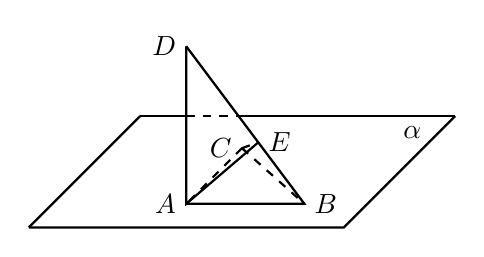
\begin{tikzpicture}[thick]
        \draw (-1,0) -- (3,0) --++ (45:2) coordinate (R);
        \draw (-1,0) --++ (45:2) coordinate (P);
        \path [name path = aboveline] (P) -- (R);
        \draw (1,0.3) node [left] {$A$} coordinate (A) -- (2.5,0.3) node [right] {$B$} coordinate (B) -- (1,2.3) node [left] {$D$} coordinate (D);
        \draw ($(B)!{16/41}!(D)$) node [right] {$E$} coordinate (E) -- (A) -- (D);
        \path [name path = A--D] (A) -- (D);
        \path [name path = B--D] (B) -- (D);
        \path [name intersections = {of = aboveline and A--D, by = U}];
        \path [name intersections = {of = aboveline and B--D, by = V}];
        \draw [dashed] (U) -- (V);
        \draw (P) -- (U) (V) -- (R);
        \draw [dashed] (A) ++ (45:1) node [left] {$C$} coordinate (C) -- (A) (C) -- (E) (C) -- (B); 
        \draw (R) --++ (-0.3,0) node [below left] {$\alpha$};
    \end{tikzpicture}
\end{center}

\begin{center}
    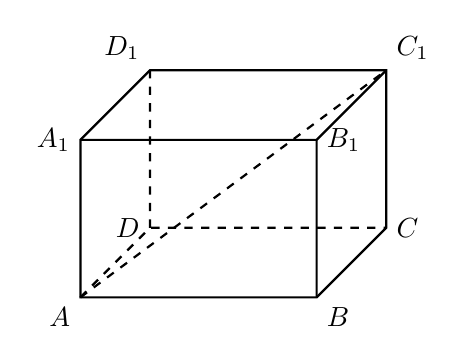
\begin{tikzpicture}[thick]
        \draw (0,0) node [below left] {$A$} coordinate (A) --++ (3,0) node [below right] {$B$} coordinate (B) --++ (45:{2.5/2}) node [right] {$C$} coordinate (C)
        --++ (0,2) node [above right] {$C_1$} coordinate (C1)
        --++ (-3,0) node [above left] {$D_1$} coordinate (D1) --++ (225:{2.5/2}) node [left] {$A_1$} coordinate (A1) -- cycle;
        \draw (A) ++ (3,2) node [right] {$B_1$} coordinate (B1) -- (B) (B1) --++ (45:{2.5/2}) (B1) --++ (-3,0);
        \draw [dashed] (A) --++ (45:{2.5/2}) node [left] {$D$} coordinate (D) --++ (3,0) (D) --++ (0,2);
        \draw [dashed] (A) -- (C1);
    \end{tikzpicture}
\end{center}

\begin{center}
    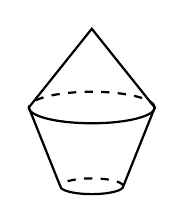
\begin{tikzpicture}[thick]
        \draw (0.4,0) -- (0.8,1) -- (0,2) -- (-0.8,1) -- (-0.4,0);
        \draw (0.4,0) arc (0:-180:0.4 and 0.1) (0.8,1) arc (0:-180:0.8 and 0.2);
        \draw [dashed] (0.4,0) arc (0:180:0.4 and 0.1) (0.8,1) arc (0:180:0.8 and 0.2);
    \end{tikzpicture}
\end{center}

\begin{center}
    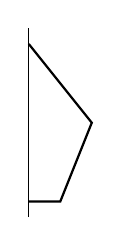
\begin{tikzpicture}[thick]
        \draw [thin] (0,-0.2) -- (0,2.2);
        \draw (0,0) -- (0.4,0) -- (0.8,1) -- (0,2);
    \end{tikzpicture}
\end{center}

\begin{center}
    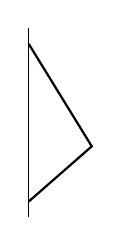
\begin{tikzpicture}[thick]
        \draw [thin] (0,-0.2) -- (0,2.2);
        \draw (0,0) -- (0.8,0.7) -- (0,2);
    \end{tikzpicture}
\end{center}

\begin{center}
    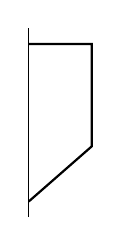
\begin{tikzpicture}[thick]
        \draw [thin] (0,-0.2) -- (0,2.2);
        \draw (0,0) -- (0.8,0.7) -- (0.8,2) -- (0,2);
    \end{tikzpicture}
\end{center}

\begin{center}
    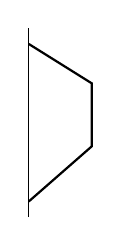
\begin{tikzpicture}[thick]
        \draw [thin] (0,-0.2) -- (0,2.2);
        \draw (0,0) -- (0.8,0.7) -- (0.8,1.5) -- (0,2);
    \end{tikzpicture}
\end{center}

\begin{center}
    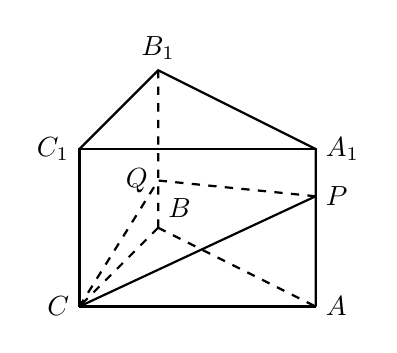
\begin{tikzpicture}[thick]
        \draw (0,0) node [left] {$C$} coordinate (C) -- (3,0) node [right] {$A$} coordinate (A);
        \draw [dashed] (1,1) node [above right] {$B$} coordinate (B) -- (A) (B) -- (C) (B) --++ (0,2) node [above] {$B_1$} coordinate (B1);
        \draw (A) --++ (0,2) node [right] {$A_1$} coordinate (A1) -- (B1) -- (0,2) node [left] {$C_1$} coordinate (C1); 
        \draw (C) -- (C1) -- (A1);
        \draw ($(A)!0.7!(A1)$) node [right] {$P$} coordinate (P) -- (C);
        \draw [dashed] (P) -- ($(B)!0.3!(B1)$) node [left] {$Q$} -- (C);
    \end{tikzpicture}
\end{center}

\begin{center}
    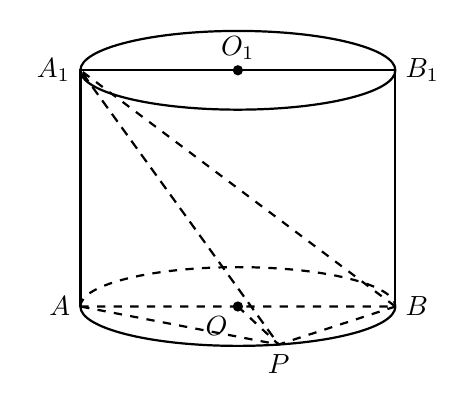
\begin{tikzpicture}[thick]
        \draw (0,0) node [left] {$A$} -- (0,3) node [left] {$A_1$} -- (4,3) node [right] {$B_1$} -- (4,0) node [right] {$B$};
        \draw (0,0) arc (180:360:2 and 0.5) (0,3) arc (180:360:2 and 0.5) (0,3) arc (180:0:2 and 0.5);
        \draw [dashed] (0,0) arc (180:0:2 and 0.5);
        \filldraw (2,0) circle (0.05) node [below left] {$O$} coordinate (O) (2,3) circle (0.05) node [above] {$O_1$} coordinate (O1);
        \draw [dashed] (0,0) -- (4,0) -- (0,3) -- ({2+2*cos(-75)},{0.5*sin(-75)}) node [below] {$P$} coordinate (P) (O) -- (P) -- (0,3) (4,0) -- (P) -- (0,0);
    \end{tikzpicture}
\end{center}

\begin{center}
    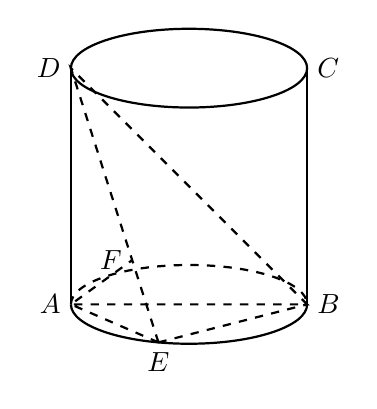
\begin{tikzpicture}[thick]
        \draw (0,0) node [left] {$A$} -- (0,3) node [left] {$D$} coordinate (D) (3,3) node [right] {$C$} -- (3,0) node [right] {$B$};
        \draw (0,0) arc (180:360:1.5 and 0.5) (0,3) arc (180:-180:1.5 and 0.5);
        \draw [dashed] (0,0) arc (180:0:1.5 and 0.5);
        \draw [dashed] ({1.5+1.5*cos(-105)},{0.5*sin(-105)}) node [below] {$E$} coordinate (E) -- (0,0) (E) -- (3,0) (E) -- (0,3) -- (3,0) -- (0,0) -- ($(E)!0.3!(D)$) node [left] {$F$};
    \end{tikzpicture}
\end{center}

\begin{center}
    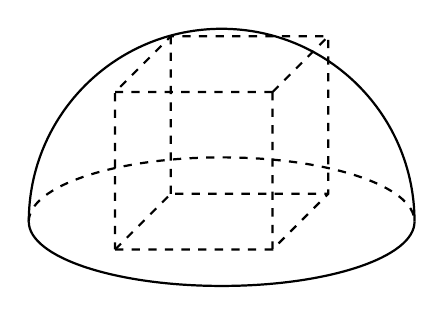
\begin{tikzpicture}[thick]
        \draw [dashed] (0,0)  coordinate (A) --++ (2,0)  coordinate (B) --++ (45:{2/2})  coordinate (C)
        --++ (0,2)  coordinate (C1) --++ (-2,0)  coordinate (D1) --++ (225:{2/2}) coordinate (A1) -- cycle;
        \draw [dashed] (A) ++ (2,2) coordinate (B1) -- (B) (B1) --++ (45:{2/2}) (B1) --++ (-2,0);
        \draw [dashed] (A) --++ (45:{2/2})  coordinate (D) --++ (2,0) (D) --++ (0,2);        
        \draw ($(A)!0.5!(C)$) ++ ({-sqrt(6)},0) coordinate (L)  arc (180:0:{sqrt(6)});
        \draw (L) arc (-180:0:{sqrt(6)} and {sqrt(6)/3});
        \draw [dashed] (L) arc (180:0:{sqrt(6)} and {sqrt(6)/3});
    \end{tikzpicture}
\end{center}

\begin{center}
    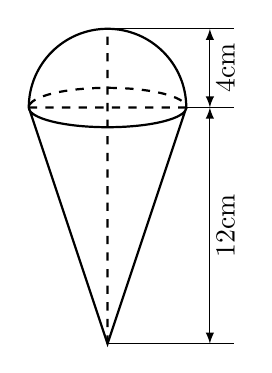
\begin{tikzpicture}[thick,>=latex]
        \draw (-1,0) -- (0,-3) -- (1,0) arc (0:180:1) arc (180:360:1 and 0.25);
        \draw [dashed] (0,-3) -- (0,1) (-1,0) -- (1,0) arc (0:180:1 and 0.25);
        \draw [thin] (1,0) -- (1.6,0) (0,-3) -- (1.6,-3) (0,1) -- (1.6,1);
        \draw [thin,<->] (1.3,0) -- (1.3,1);
        \draw [thin,<->] (1.3,0) -- (1.3,-3);
        \draw (1.5,0.5) node {\rotatebox{90}{$4\text{cm}$}};
        \draw (1.5,-1.5) node {\rotatebox{90}{$12\text{cm}$}};
    \end{tikzpicture}
\end{center}

\begin{center}
    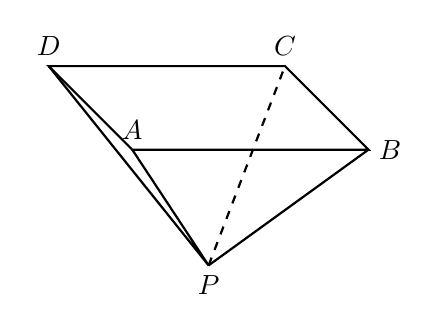
\begin{tikzpicture}[thick]
        \draw (0,0) node [above] {$A$} -- (3,0) node [right] {$B$} coordinate (B) --++ (135:1.5) node [above] {$C$} coordinate (C) --++ (-3,0) node [above] {$D$} coordinate (D) -- cycle;
        \draw ($(B)!0.5!(D)$) ++ (0,-2) node [below] {$P$} coordinate (P) (P) -- (0,0) (P) -- (D) (P) -- (B);
        \draw [dashed] (P) -- (C);
    \end{tikzpicture}
\end{center}

\begin{center}
    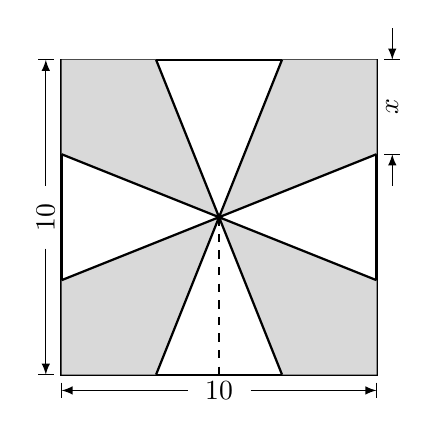
\begin{tikzpicture}[thick,>=latex]
        \draw (-2,-2) -- (-2,2) -- (2,2) -- (2,-2) -- cycle;
        \fill [gray!30] (0,0) -- (0.8,2) -- (2,2) -- (2,0.8) -- cycle;
        \fill [gray!30] (0,0) -- (-0.8,2) -- (-2,2) -- (-2,0.8) -- cycle;
        \fill [gray!30] (0,0) -- (0.8,-2) -- (2,-2) -- (2,-0.8) -- cycle;
        \fill [gray!30] (0,0) -- (-0.8,-2) -- (-2,-2) -- (-2,-0.8) -- cycle;
        \draw (0.8,-2) -- (-0.8,2) (-0.8,-2) -- (0.8,2) (-2,0.8) -- (2,-0.8) (-2,-0.8) -- (2,0.8);
        \draw [dashed] (0,0) -- (0,-2);
        \draw [thin] (-2,-2.1) -- (-2,-2.3) (2,-2.1) -- (2,-2.3) (-2.1,-2) -- (-2.3,-2) (-2.1,2) -- (-2.3,2) (2.1,2) -- (2.3,2) (2.1,0.8) -- (2.3,0.8);
        \draw [->,thin] (-0.4,-2.2) -- (-2,-2.2);
        \draw [->,thin] (0.4,-2.2) -- (2,-2.2);
        \draw [->,thin] (-2.2,-0.4) -- (-2.2,-2);
        \draw [->,thin] (-2.2,0.4) -- (-2.2,2);
        \draw [->,thin] (2.2,0.4) -- (2.2,0.8);
        \draw [->,thin] (2.2,2.4) -- (2.2,2);
        \draw (0,-2.2) node {$10$} (-2.2,0) node {\rotatebox{90}{$10$}} (2.2,1.4) node {\rotatebox{90}{$x$}};
    \end{tikzpicture}
\end{center}

\begin{center}
    \begin{tikzpicture}[thick]
        \draw (0,0) node [left] {$A$} -- (3,0) node [right] {$B$} coordinate (B) --++ (45:1.5) node [right] {$C$} coordinate (C) ++ (-3,0) node [below right] {$D$} coordinate (D);
        \draw ($(B)!0.5!(D)$) node [below left] {$O$} coordinate (O) ++ (0,2) node [above] {$E$} coordinate (E) (E) -- (0,0) (E) -- (C) (E) -- (B);
        \draw [dashed] (E) -- (D);
        \draw [dashed] ($(B)!0.5!(C)$) node [right] {$F$} coordinate (F) -- (O) -- (E) (C) -- (D) -- (A);
        \draw (E) -- (F);
    \end{tikzpicture}
\end{center}

\begin{center}
    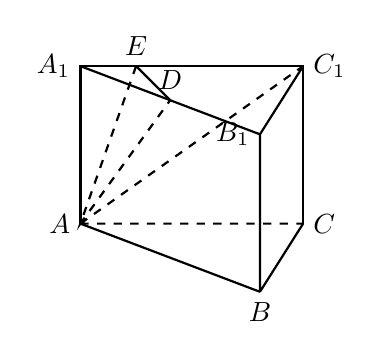
\begin{tikzpicture}[thick]
        \draw (0,0) node [left] {$A$} coordinate (A) -- (0,2) node [left] {$A_1$} coordinate (A1) --++ ({2*sqrt(2)},0) node [right] {$C_1$} coordinate (C1) --++ (0,-2) node [right] {$C$} coordinate (C);
        \draw ({sqrt(2)},0) ++ (-45:{sqrt(6)/2}) node [below] {$B$} coordinate (B) --++ (0,2) node [left] {$B_1$} coordinate (B1) (B) -- (A) (B) -- (C) (B1) -- (A1) (B1) -- (C1);
        \draw ($(A1)!0.5!(B1)$) node [above] {$D$} coordinate (D) -- ($(A1)!0.25!(C1)$) node [above] {$E$} coordinate (E);
        \draw [dashed] (E) -- (A) -- (D) (A) -- (C1) (A) -- (C);
    \end{tikzpicture}
\end{center}

\begin{center}
    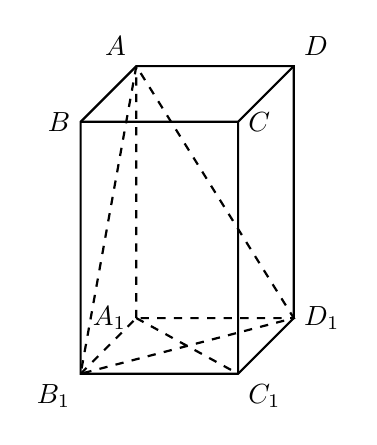
\begin{tikzpicture}[thick,scale = 2]
        \draw (0,0) node [below left] {$B_1$} coordinate (B1) --++ (1,0) node [below right] {$C_1$} coordinate (C1) --++ (45:{1/2}) node [right] {$D_1$} coordinate (D1)
        --++ (0,1.6) node [above right] {$D$} coordinate (D)
        --++ (-1,0) node [above left] {$A$} coordinate (A) --++ (225:{1/2}) node [left] {$B$} coordinate (B) -- cycle;
        \draw (B1) ++ (1,1.6) node [right] {$C$} coordinate (C) -- (C1) (C) --++ (45:{1/2}) (D) (C) --++ (-1,0);
        \draw [dashed] (B1) --++ (45:{1/2}) node [left] {$A_1$} coordinate (A1) --++ (1,0) (A1) --++ (0,1.6);
        \draw [dashed] (A) -- (B1) -- (D1) -- cycle (A1) -- (C1);
    \end{tikzpicture}
\end{center}

\begin{center}
    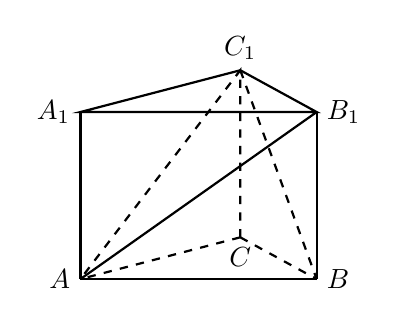
\begin{tikzpicture}[thick,scale = 1.5]
        \draw (0,0) node [left] {$A$} coordinate (A) -- (2,0) node [right] {$B$} coordinate (B);
        \draw [dashed] (1,0) ++ (45:0.5) node [below] {$C$} coordinate (C) -- (A) (C) -- (B) (C) --++ (0,{sqrt(2)}) node [above] {$C_1$} coordinate (C1) -- (A) (C1) -- (B);
        \draw (A) --++ (0,{sqrt(2)}) node [left] {$A_1$} coordinate (A1) (B) --++ (0,{sqrt(2)}) node [right] {$B_1$} coordinate (B1);
        \draw (A1) -- (B1) -- (C1) -- cycle (A) -- (B1);
    \end{tikzpicture}
\end{center}
\end{enumerate}
\end{document}

